% UTF-8

% single-chapter commands
\documentclass[../main/thesis.tex]{subfiles}
\onlyinsubfile{\setcounter{chapter}{5}}  % single-chapter command
\begin{document}


\chapter{Ergebnisdiskussion}
\label{ch:result}
% alles NUR im "Anwendungskontext", d.h. in Bezug auf die Ausgabe-Geodaten, nicht die Softwarequalität (das war in 5.4!)

%Die in Kap. 4 und 5 entwickelte Software ist das Ergebnis dieser Arbeit. Hier diskutiert werden soll die Arbeitsweise dieser Software und die Qualität der von ihr ausgegebenen Geodaten in Bezug auf die Aufgabenstellung.

Bei der Evaluierung der Software ist zu bedenken, dass die \osm-Datenbank ständig bearbeitet wird.
Konsistente Ergebnisse für ein bestimmtes Gebiet erfordern daher, dass immer mit Geodaten vom selben Stand gearbeitet wird.

In diesem Kapitel wird nach und nach anhand von Einzelbeispielen die Funktion der mit dieser Arbeit entwickelten Software (dem \term{Combiner}) besprochen.
Die genutzten Geodaten für das Straßennetz beschränken sich auf einen Testdatensatz aus \osm\ für das Land Nordrhein-Westfalen vom November~2012.
% http://dev.thaw.de/temp/highways/nrw-roads.zip (testbed-nrw-prepare.sh)

Anhänge~\ref{appx:fullpage-examples-1} und~\ref{appx:fullpage-examples-2} zeigen weitere Beispiele der Anwendung des \term{Combiners} auf aktuelle Geodaten größerer zusammenhängender Areale auch in anderen Regionen.



\section{Anwendung in einfachen Situationen}
\label{ch:result-trivial}

Bei Anwendung des \term{Combiners} auf Geodaten aus der \osm-Datenbank zeigt sich, dass die implementierten Algorithmen grundsätzlich funktionieren.

\onefigure{p}{
	\twofigures{H}{
		\begin{overpic}[width=\ScaleIfNeeded]{../chapter6/result-trivial-in}
			\put(122,84){\figuremark{1}}
			\put(58,60){\figuremark{2}}
			\put(23,39){\rotatebox{50}{\figureframe{.1167}}}
		\end{overpic}
	}{
		\begin{overpic}[width=\ScaleIfNeeded]{../chapter6/result-trivial-out}
			\put(122,84){\figuremark{1}}
			\put(58,60){\figuremark{2}}
			\put(23,39){\rotatebox{50}{\figureframe{.1167}}}
		\end{overpic}
	}
	% trivial = testbed-nrw/koeln-classfied-nolinks.shp
	% 1:30000 Google Mercator, bbox 778765 6607045 780865 6608245, 0.2mm stroke
	\caption{Ergebnis des \term{Combiners} im einfachen Fall (links Eingangsdaten, rechts Generalisierungsergebnis; Köln-Gremberg mit Autobahn L\,124)}
	\label{fig:result-trivial}
}

In Abbildung~\ref{fig:result-trivial} sind links \osm-Linienzüge in der einfachen Situation einer Autobahn ohne Anschlussstellen nebst innerstädtischen Sammelstraßen zu sehen.
Durch Anwendung des \term{Combiners} ergibt sich das rechts dargestellte automatisiert zusammengefasste Ergebnis.
Anstelle der beiden Richtungsfahrbahnen der Autobahn gibt es nun nur noch einen einzigen Linienzug als Straßenachse.
Die Nähe zu nachgeordneten Straßen und deren planfreie Kreuzung mit der Autobahn (bei Markierung~\textfiguremark{1}) stört die Generalisierung nicht.
Auch eine Strecke paralleler Fahrbahnen im nachgeordneten Netz wurde trotz eines scharfen Knicks erfolgreich als parallel erkannt und zusammengefasst (Markierung~\textfiguremark{2}).

\onefigure{p}{
	\twofigures{H}{
		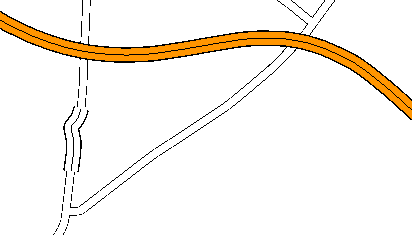
\includegraphics[width=\ScaleIfNeeded]{../chapter6/result-trivial-styled}
	}{
		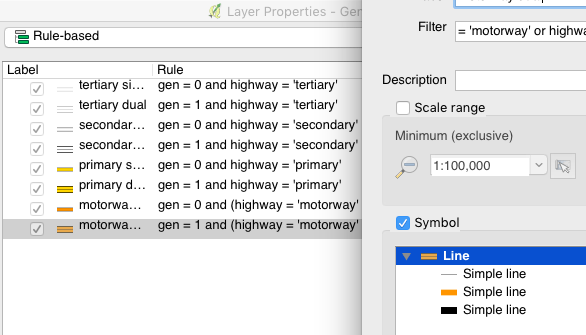
\includegraphics[width=\ScaleIfNeeded]{../chapter6/result-trivial-rules}
	}
	\caption{Visualisierung des Generalisierungsergebnisses (links Kartendarstellung, rechts Screenshot der Zeichenregeln in QGIS)}
	\label{fig:result-trivial-styled}
}

Abbildung~\ref{fig:result-trivial-styled} zeigt beispielhaft, wie sich dieses Generalisierungsergebnis sinnvoll visualisieren ließe.
Der \term{Combiner} kennzeichnet die zusammengefassten Linienzüge als generalisiert.
Zusätzlich gibt der \term{Combiner} einzelne \term{tags} der \osm-Quelldaten mit aus.
Anhand dieser Attribute können leicht Regeln mit jeweils passenden Linearsignaturen definiert werden.

% writeNodeMatches
\onefigure{p}{
	\twofigures{H}{
		\begin{overpic}[width=\ScaleIfNeeded]{../chapter6/result-trivial-detail-rolshover}
			\put(129,0){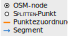
\includegraphics{../chapter6/legend-nodematch}}
			\put(53,7){\figuremark{1}}
			\put(81,85){\figuremark{2}}
			\put(184,83){\figuremark{3}}
		\end{overpic}
	}{
		\begin{overpic}[width=\ScaleIfNeeded]{../chapter6/result-trivial-detail-rolshover-gen}
			\put(129,0){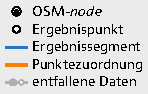
\includegraphics{../chapter6/legend-nodematch-gen}}
			\put(53,7){\figuremark{1}}
			\put(81,85){\figuremark{2}}
			\put(184,83){\figuremark{3}}
		\end{overpic}
	}
	% 1:3500 Google Mercator rotated 50°, bbox 779025 6607525 779270 6607665
	\caption{Detaildarstellung Generalisierung mit Punktezuordnungen (links Eingangsdaten, rechts Generalisierungsergebnis; \textfiguremark{2}~in Abbildung~\ref{fig:result-trivial})}
	\label{fig:result-trivial-detail-rolshover}
}

Bei näherer Betrachtung ist die korrekte Arbeitsweise der implementierten Algorithmen in diesem einfachen Fall gut zu erkennen (Abbildung~\ref{fig:result-trivial-detail-rolshover}):
Linienzüge werden durch \textproc{Splitten} derart unterteilt, dass möglichst jeweils zwei Punkte auf Parallelen einander gegenüber liegen (gut zu sehen bei~\textfiguremark{1}).
Die dabei entstehenden einander gegenüberliegenden Fragmente sind durch ihre Ähnlichkeit offensichtlich einfach auf Parallelität zu prüfen.
Selbst dann, wenn beim \textproc{Splitten} keine optimalen Paare entstehen, gelingt dies, solange wenigstens jeweils ein \emph{Teil} der miteinander verglichenen Segmente zueinander parallel ist (\textfiguremark{2}).
Von den so entstehenden Zuordnungen der einander gegenüberliegenden \osm-\term{nodes} lässt sich durch Verbindung ihrer Mittelpunkte leicht eine Mittellinie im Verlauf der Straßenachse als Ergebnis ableiten.

Der Übergang zwischen generalisierten und nicht generalisierten Linienzügen (\textfiguremark{3}) wird unten im Abschnitt~\ref{ch:relocateGeneralisedNodes} diskutiert.

Für den NRW-Testdatensatz wurden die in Abschnitt~\ref{ch:analyse-algorithm} genannten Beispielwerte von höchstens um $15\degree$ abweichender Ausrichtung und höchstens $\unit[40]{m}$ Abstand zweier \textproc{Parallel}er Segmente empirisch als grundsätzlich tauglich bestätigt.
% evtl. näher ausführen, Tabelle mit Zahlen machen, ...
Für Autobahnen genügt überwiegend bereits ein Limit von nur $10\degree$ Abweichung.
Sonstige Straßen besitzen wesentlich engere Kurvenradien und haben dabei vereinzelt Segmente, welche als parallel gelten könnten, deren Ausrichtung jedoch um $30\degree$ oder mehr voneinander abweicht.

% Ausrichtungsgrenze 15°:
% - empirisch ermittelter vernünftiger Bereich für autobahnähnlich etwa 8..16°
% - empirisch ermittelter vernünftiger Bereich für innerstädtisch etwa 20..40°

% Distanz 40 m:
% - empirisch ermittelter vernünftiger Bereich für autobahnähnlich etwa 40..45 m
% - empirisch ermittelter vernünftiger Bereich für innerstädtisch etwa 35..50 m

Um Praxistauglichkeit zu erreichen, müsste die Definition von \textproc{Parallel} folglich vom Straßentyp abhängen.
Dies wurde aus Zeitgründen nicht mehr als Teil dieser Arbeit umgesetzt.

Der NRW-Testdatensatz enthält als \osmtag{highway}[motorway] attributierte Linienzüge mit einer Gesamtlänge von $\unit[4515]{km}$.
% roads-motorway.shp
Der \term{Combiner} erkennt $\unit[4461]{km}$ davon als parallel; das ausgegebene Ergebnis besteht auf $\unit[97,6]{\%}$ Länge aus zusammengefassten Linienzügen.
Nachdem alle nordrhein-westfälischen Autobahnen zweibahnig ausgebaut sind, wäre bei naiver Betrachtung eine Erkennungsrate von $\unit[100]{\%}$ zu erwarten gewesen.
Die Untersuchung der ausgegebenen Ergebnisdaten hat gezeigt, dass Linienzüge im Wesentlichen in den folgenden Fällen als \emph{nicht} parallel erkannt werden:

\begin{itemize}[nosep]
\item fehlerhafte Klassifizierung von Auf- und Abfahrten (\osmtag{highway}[*])
% (insb. \osmtag{highway}[motorway] statt \term{motorway\_link})
\item fehlerhaftes Attribut für die Straßennummer (\osmtag{ref}[*])
% \osmtag{ref} einseitig fehlend oder voneinander abweichend
\item definierte geometrische Kriterien für Parallelität nicht erfüllt \\(z.~B. ungewöhnlich großer Abstand der Richtungsfahrbahnen)
\end{itemize}
%
Letzteres ist zu erwarten und offensichtlich korrekt.
Die ersten beiden Fälle werden in den folgenden Abschnitten~\ref{ch:result-tags} und~\ref{ch:result-junctions} näher betrachtet.



\section{Berücksichtigung von Attributen}
\label{ch:result-tags}

Die in Abschnitt~\ref{ch:analyse-algorithm} beschriebenen Algorithmen berücksichtigen neben der Klassifizierung der Straße als einziges Attribut die Straßennummer.
% in der Annahme, dass diese normalerweise stimmt
Im NRW-Testdatensatz erkennt der \term{Combiner} $\unit[54]{km}$ der Autobahn-Fahrbahnen nicht als parallel; wird die Straßennummer nicht berücksichtigt, sinkt diese Länge auf $\unit[31]{km}$.

An mehreren der dann neu erkannten Stellen trägt nur eine der beiden Richtungsfahrbahn die Straßennummer als Attribut.
In Abschnitt~\ref{ch:case-selection} wurde dargelegt, dass im Straßennetz grundsätzlich eine vergleichsweise hohe Datenqualität zu erwarten gewesen wäre, weil Fehler darin in der Standard-Karte auf \href{https://www.openstreetmap.org/}{\nolinkurl{osm.org}} störend sichtbar sind und deswegen zügig von \osm-Beitragenden behoben werden.
Die nur für \emph{eine} Richtungsfahrbahn fehlende Straßennummer fällt jedoch dem Beitragenden nicht unbedingt auf, solange die Straßennummer der \emph{anderen} Richtungsfahrbahn korrekt angezeigt wird.

Vereinzelt existieren allerdings sogar widersprüchliche Straßennummern der beiden Richtungsfahrbahnen.
So ist auf mehreren Abschnitten bei Dülmen die eine Fahrbahn \osmtag{ref}[A\,43] gekennzeichnet, die andere jedoch \osmtag{ref}[A\,43;B\,474]; bei Bliesheim trägt eine der Richtungsfahrbahnen der A\,553 das Attribut \osmtag{ref}[A\,1].

Da in diesen Fällen die Geometrie der Fahrbahnen offensichtlich parallel ist, muss hinterfragt werden, welche Bedeutung den Attributen beigemessen werden sollte.
Der \term{Combiner} berücksichtigt derzeit entgegen der ursprünglichen Definition standardmäßig nicht mehr die Straßennummer.
%Auch dies könnte jedoch zu Problemen führen, weil damit zwei Fahrbahnen gleicher Klassifizierung, die nur zufällig parallel sind, jedoch zu unterschiedlichen Straßen gehören, fälschlich als Richtungsfahrbahnen derselben Straße erkannt werden könnten.
Dieses Verhalten kann mit dem Schalter \texttt{--tags} kontrolliert werden.



\section{Verhalten an Straßenkreuzungen}
\label{ch:result-junctions}

\subsection{Beseitigung von Topologielücken}
\label{ch:relocateGeneralisedNodes}

Beim Zusammenfassen von Linienzügen erzeugt der \term{Combiner} neue Stützpunkte entlang einer Mittellinie.
Werden die Stützpunkte der ursprünglichen Linienzüge noch für weitere Zwecke verwendet, dürfen diese nicht entfallen, sondern müssen erhalten bleiben.

An \term{nodes}, die sowohl beim Zusammenfassen entfallene Linien als auch andere Linien benutzen, wird dies zum Problem:
Sie werden von nicht generalisierten Linien weiterbenutzt, die generalisierten Linien hingegen verwenden die neu erzeugten Punkte, so dass an den Übergängen topologische Lücken im Straßennetz entstehen.
Der \term{Combiner} versucht dem zu begegnen, indem die \term{nodes} an den Enden \emph{nicht} generalisierter Linienzüge auf diese Situation hin geprüft und nötigenfalls durch geeignete Punkte auf der generalisierten Mittellinie ersetzt werden.

\onefigure{h}{
	\twofigures{H}{
		\begin{overpic}[width=\ScaleIfNeeded]{../chapter6/koelnarena-gen}
			\put(0,0){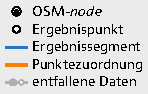
\includegraphics{../chapter6/legend-nodematch-gen}}
			\put(51,67){\figuremark{1}}
			\put(137,24){\figuremark{2}}
		\end{overpic}
	}{
		\begin{overpic}[width=\ScaleIfNeeded]{../chapter6/koelnarena-gen-cleanup}
			\put(0,0){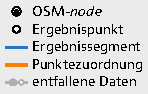
\includegraphics{../chapter6/legend-nodematch-gen}}
			\put(51,67){\figuremark{1}}
			\put(137,24){\figuremark{2}}
		\end{overpic}
	}
	% 1:5500 Google Mercator, bbox 777275 6610050 777660 6610270
	\caption{Detaildarstellung der Beseitigung von Topologielücken (links vorher, rechts nachher; L\,111 in Köln-Deutz)}
	\label{fig:koelnarena-gen-cleanup}
}

Abbildung~\ref{fig:koelnarena-gen-cleanup} zeigt, dass diese Lösung grundsätzlich funktioniert.
Die Straßenkreuzung bei \textfiguremark{1} wird auf einen einzelnen Punkt zusammengefasst, so dass beide Straßen korrekt miteinander verknüpft sind.
Auch der bereits in Abschnitt~\ref{ch:generalisation-algorithm} angesprochene und zunächst offen gelassene Übergang eines einzelnen Linienzugs in zwei parallele Linienzüge bei \textfiguremark{2} wird so gelöst.

Dieses zusätzliche, in Abschnitt~\ref{ch:algorithm-parts} nicht beschriebene Verfahren ist standardmäßig aktiv, kann aber mit dem Schalter \texttt{--no-cleanup} kontrolliert werden.
Auch in Abbildung~\ref{fig:result-trivial-detail-rolshover} kam es zum Einsatz.
Darin ist bei \textfiguremark{3} gut zu sehen, wie am Beginn des generalisierten Abschnitts die Geometrie geringfügig geändert wird, um die Topologie zu erhalten.

Topologielücken können jedoch nur dann mit diesem Verfahren geschlossen werden, wenn tatsächlich ein \emph{geeigneter} Punkt auf der generalisierten Mittellinie gefunden wird.
Wie die folgenden Abschnitte zeigen werden, ist dies oft nicht der Fall.
%Wird ein \emph{un}geeigneter Punkt gefunden, entstehen spitzwinklige Haken (siehe Anhang~\ref{appx:junction-examples}, Abbildung XYZ), Segmente mit Nulllänge usw. usf.

Mit diesem Verfahren können überdies in der gegenwärtigen Implementierung nur solche Topologielücken beseitigt werden, die erst beim Zusammenfassen von Parallelen entstanden sind.
Besonders auffallend ist diese Einschränkung bei Verbindungsrampen an planfreien Kreuzungen.
Sie sind keine Richtungsfahrbahnen und werden deshalb wie in Abschnitt~\ref{ch:case-selection} festgelegt in dieser Arbeit nicht betrachtet.
Sie sind deshalb bereits in den Eingangsdaten für die Zusammenfassung durch Objektauswahl entfallen und damit auch nicht im Generalisierungsergebnis enthalten (Abbildung~\ref{fig:breitscheid-gen-styled}).

Dass einander kreuzende Autobahnen miteinander verknüpft sind, lehrt die Lebenserfahrung; aus der Topologie der generalisierten Geodaten geht es indes nicht hervor.

\onefigure{h}{
	\begin{overpic}[width=7cm]{../chapter6/breitscheid-bg}
		\put(0,0){\scalebox{1}[1.0008]{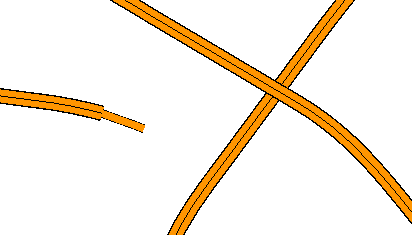
\includegraphics[width=7cm]{../chapter6/breitscheid-gen-styled}}}
	\end{overpic}
	% 1:50000 Google Mercator, bbox 761000 6682100 764500 6684100
	\caption{Fehlende Verbindungsrampen im Generalisierungsergebnis ~~~~~~~~~~~~~~~~~~~~~~~~~\cf[entsättigt][Hintergrund ]{map:osm-carto}}
	\label{fig:breitscheid-gen-styled}
}



\subsection{Fehlende Kreuzungserkennung}
\label{ch:missing-junction-detection}

\onefigure{t}{
	\begin{overpic}[width=\ScaleIfNeeded]{../chapter6/kanal-gen-cleanup}
		\put(0,67.5){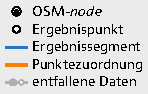
\includegraphics{../chapter6/legend-nodematch-gen}}
		\put(168,35){\figuremark{1}}
		\put(161,85){\figuremark{2}}
		\put(107,33){\figuremark{3}}
	\end{overpic}
	% 1:3500 Google Mercator rotated 10°, bbox 771595 6612098 771840 6612238
	\caption{Verbleibende Topologielücken (Innere Kanalstraße, Köln)}
	\label{fig:kanal-gen-cleanup}
}

Das in Abschnitt~\ref{ch:relocateGeneralisedNodes} beschriebene Verfahren funktioniert auch innerstädtisch nicht in jeder Situation, wie Abbildung~\ref{fig:kanal-gen-cleanup} zeigt.
Zwar führt es zu einem gelungenen Ergebnis bei \textfiguremark{1}.
Bei \textfiguremark{2} und \textfiguremark{3} wird hingegen aufgrund der spezifischen Kreuzungsgeometrie kein „geeigneter“ Punkt auf einer der generalisierten Linien gefunden.
% genauer gesagt: es werden die falschen Punkte gefunden
Die dortigen Lücken in der Topologie bleibt somit bestehen.
Ähnliche Probleme existieren an vielen weiteren innerstädtischen Kreuzungen.

Zwar ließe sich argumentieren, dass in vielen dieser Fälle die Attribute der \osm-Daten fehlerhaft sind.
Beispielsweise sollte in Abbildung~\ref{fig:kanal-gen-cleanup} die \textfiguremark{1} und \textfiguremark{3} verbindende Abbiegefahrbahn eigentlich als solche klassifiziert werden (\osmtag{highway}[primary\_link] statt \term{primary}), wodurch vermieden würde, dass sie bei \textfiguremark{3} als parallel zur Hauptfahrbahn erkannt wird. \cf{osm:HighwayLink}

Allerdings ist gerade dieser Fehler im NRW-Testdatensatz stark verbreitet.
So sind in der Kölner Innenstadt (bis einschließlich der Ringe) von insgesamt 79
% Ringe(außen) + Ringe(mittig) + Ringe(innen) + West + Nord-Süd-Fahrt + Ost:
% 6+13+15+11+26+8
Abbiegefahrbahnen ganze 26
% 2+3+6+5+9+1
nicht als solche klassifiziert.
Es ist auch fraglich, ob hier mit fortschreitender Bearbeitung der \osm-Datenbank Verbesserungen zu erwarten sind, denn Abbiegefahrbahnen und Hauptfahrbahnen werden auf \href{https://www.openstreetmap.org/}{\nolinkurl{osm.org}} mit nahezu identischer Linearsignatur gezeichnet, so dass eine falsche Klassifizierung beim Betrachten nicht auffällt.
% gemeint ist der Effekt, dass crowdgesourcte VGI im Laufe der Zeit zu Korrektheit tendiert
Vor dem Hintergrund der Aufgabenstellung, die das Ziel \emph{praxistauglicher} Algorithmen vorgibt, ist folglich offensichtlich, dass dieses Problem einer automatisierten Lösung bedarf.

An Kreisverkehren gibt es ebenfalls typische Probleme.
Abbildung~\ref{fig:roundabout-gen-cleanup} zeigt, wie alle im Kreis einander gegenüberliegenden Segmente als parallel erkannt werden.
Mit dieser Masse widersprüchlicher Punktezuordnungen kann der Algorithmus zur Zusammenfassung keine brauchbaren Ergebnisse mehr liefern.
Auch der in Abschnitt~\ref{ch:relocateGeneralisedNodes} besprochene Ansatz zur Beseitigung von Lücken in der Topologie läuft ins Leere.

\onefigure{h}{
	\begin{overpic}[width=\ScaleIfNeeded]{../chapter6/roundabout-gen-cleanup}
		\put(0,0){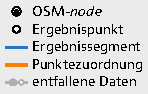
\includegraphics{../chapter6/legend-nodematch-gen}}
	\end{overpic}
	% 1:2000 Google Mercator, bbox 785968 6600972 786108 6601052
	\caption{Verhalten am Kreisverkehr (Friedrichstraße, Köln-Porz)}
	\label{fig:roundabout-gen-cleanup}
}

Zwar wäre es möglich, die meisten Kreisverkehre über \osm-\term{tags} zu erkennen und von der Generalisierung ausschließen (was aber aus Zeitgründen nicht mehr als Teil dieser Arbeit umgesetzt wurde).
% prinzipiell trivial in shouldEvaluate möglich, jedoch erfordert dies, dass die Kreisverkehr-tags vorliegen
Eine Generalisierung der Kreisverkehre -- zum~Beispiel durch Qualitätsumschlag der linearen Kreisfahrbahn in einen einzelnen Kreuzungspunkt -- könnte jedoch überaus nützlich sein, etwa bei der Herstellung einer Straßenkarte im mittleren Maßstabsbereich.

\newpage
Auffallend ist, dass alle diskutierten Probleme an Kreuzungen auftreten.
Auf freier Strecke funktioniert der \term{Combiner} weitgehend problemlos.
Gäbe es eine zuverlässige Methode, automatisiert Kreuzungen zu erkennen, ließe sich möglicherweise leicht Praxistauglichkeit erzielen.

Anhang~\ref{appx:junction-examples} zeigt weitere Beispiele von Kreuzungssituationen, mit denen der \term{Combiner} nicht gut zurechtkommt.



\section{Effizienz}

Die Implementierung der vorgestellten Algorithmen im \term{Combiner} hat bei Anwendung auf den NRW-Testdatensatz wie in Abschnitt~\ref{ch:algorithm-overview} erwartet einen Zeitaufwand, der im Verhältnis zur Zahl der Segmente nicht schneller als linear wächst.
Tabelle~\ref{tab:profiling-segments} stellt die gemessenen Ausführungszeiten $t$ am Beispiel von Fernstraßen (bis einschließlich \osmtag{highway}[primary], ohne \term{links}) in der Umgebung von Köln dar.
% wall clock ("processing time")
Angefangen mit einer Gruppe von Stadtteilen bis hin zum Bundesland Nordrhein-Westfalen wurden steigende Flächengrößen berechnet bei ansonsten gleichen Bedingungen.

\onetable{h}{
	\begin{tabular}{lrrlcccrc}
&&&& \multicolumn{2}{@{}c@{}}{Wachstumsfaktor} &&& \\
Gebiet & \multicolumn{1}{c}{Fläche} & \multicolumn{1}{c}{$|S|$} & \multicolumn{1}{c}{$t$} & für $|S|$ & für $t$ & $\frac{|S'|}{|S|}$ & \multicolumn{1}{c}{$\nu$} & $\psi$ \\
\hline\rule{0mm}{0.8\normalbaselineskip}%
Stadtteile &   161\,km$^2$ &   3516 & 0,41\,s & --  & --  & 1,56 & 10 & 1,31 \\
Großstadt  &   647\,km$^2$ &   8776 & 0,78\,s & 2,5 & 1,9 & 1,48 &  8 & 1,25 \\
Reg.-Bez.  &  7556\,km$^2$ &  54247 & 2,2\,s  & 6,2 & 2,8 & 1,23 &  8 & 1,37 \\
Bundesland & 34881\,km$^2$ & 157014 & 5,7\,s  & 2,9 & 2,6 & 1,27 &  6 & 1,27 \\
	\end{tabular}
	\caption{Zeitbedarf für unterschiedlich große Gebiete}
	\label{tab:profiling-segments}
}

Es bestätigt sich, dass die in Abschnitt~\ref{ch:algorithm-overview} eingeführten Größen $\nu$ und $\psi$ nicht von $|S|$ abhängig sind.
Der Wachstumsfaktor für $|S|$ beim Schritt von der Großstadt zum Regierungsbezirk ist mit 6,2 deutlich größer als der Faktor für $t$ mit 2,8.
Wie das Verhältnis $|S'|\nobreak:\nobreak|S|$ der Segmentanzahl nach bzw. vor dem \textproc{Splitten} zeigt, liegt dies an dem mit diesem Schritt erstmals inkludierten ländlichen Raum.
Auch dies entspricht den Erwartungen.

\onetable{b}{
	\begin{tabular}{lcrcccrc}
&&& \multicolumn{2}{@{}c@{}}{Wachstumsfaktor} &&& \\
\term{links} & $|S|$ & \multicolumn{1}{c}{$t$} & für $|S|$ & für $t$ & $\frac{|S'|}{|S|}$ & \multicolumn{1}{c}{$\nu$} & $\psi$ \\
\hline\rule{0mm}{0.8\normalbaselineskip}%
ohne & 54247 & 2,2\,s  & --  & --  & 1,23 &  8 & 1,37 \\
mit & 73408 & 12,8\,s & 1,4 & 5,9 & 1,85 & 11 & 1,42 \\
	\end{tabular}
	\caption{Zeitbedarf ohne und mit Verbindungsfahrbahnen}
	\label{tab:profiling-links}
}

Wird neben der Segmentanzahl in den Eingangsdaten auch deren Detaillierungsgrad geändert, ergibt sich jedoch ein anderes Bild.
Tabelle~\ref{tab:profiling-links} zeigt das Verhalten des \term{Combiners} beim Hinzufügen von Abbiege- und Verbindungsfahrbahnen \term{(links)}.
Der Zeitbedarf wächst hier überproportional.
Dem deutlich gestiegenen Verhältnis $|S'|\nobreak:\nobreak|S|$ zufolge könnte dies an dem bereits in Abschnitt~\ref{} angedeuteten hohen Speicheraufwand der gewählten Implementierung liegen.

Auch dies ist ein deutlicher Hinweis auf die oben diskutierte Notwendigkeit einer Kreuzungserkennung.

% durch Spectre/Meltdown keine großen Einbußen zu erwarten, weil die Berechnung hauptsächlich im RAM stattfindet und somit der Kernel keine große Rolle spielt



\section{Anwendung auf andere Spezialfälle}
\label{ch:result-other-cases}

Der nach Abschnitt~\ref{ch:case-selection} zu untersuchende Spezialfall von \emph{Richtungs}fahrbahnen impliziert, dass die entwickelten Algorithmen genau zwei entgegengerichtete Fahrbahnen derselben Straße zusammenzufassen sollen.
Ebenda wurde jedoch bereits angedeutet, dass sie möglicherweise auch auf andere Spezialfälle anwendbar sein könnten.
Abschließend soll deshalb an zwei Beispielen betrachtet werden, wie sich die im \term{Combiner} implementierten Algorithmen verhalten, wenn die Eingangsdaten nicht entsprechend dem Spezialfall aufgebaut sind, für den die Algorithmen entwickelt wurde.



\subsection{Fahrbahnen für unterschiedliche Arten von Verkehr}
%\label{ch:result-iterated-execution}

Verteilerfahrbahnen und langgezogene Rampen für abbiegenden Verkehr sind verbreitete, schon in Abschnitt~\ref{ch:different-traffic-types-case-desc} genannte Beispiele für parallele Fahrbahnen für unterschiedliche Verkehrsarten.

Nachdem der \term{Combiner} dazu vorgesehen ist, $n$~parallele Linienzüge zu $n-1$~Linienzügen zu generalisieren (mit $n=2$ im Normalfall), liegt es nahe, die Algorithmen zur Generalisierung einfach $n-1$~Mal nacheinander anzuwenden, so dass im besten Fall auch bei beliebig vielen Parallelen am Ende nur noch ein einziger Linienzug übrig bleibt.
Abbildung~\ref{fig:iteration-good} demonstriert, dass diese Strategie gelingen könnte.

\onefigure{h}{
	\twofigures{H}{
		\begin{overpic}[width=\ScaleIfNeeded]{../chapter6/opladen-gen-1}
			\put(0,0){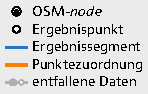
\includegraphics{../chapter6/legend-nodematch-gen}}
		\end{overpic}
	}{
		\begin{overpic}[width=\ScaleIfNeeded]{../chapter6/opladen-gen-2}
			\put(0,0){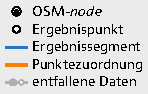
\includegraphics{../chapter6/legend-nodematch-gen}}
		\end{overpic}
	}
	% 1:6500 Google Mercator rotated -24°, bbox 778845 6630050 779300 6630310
	\caption{Detaildarstellung der wiederholten Ausführung für mehr als zwei Parallele (links erste, rechts zweite Generalisierung; A\,3 bei Leverkusen)}
	\label{fig:iteration-good}
}

Wie zu sehen ist, wird in diesem Beispiel die zwischen $2$ und $3$ variierende Zahl von Parallelen in zwei Schritten korrekt auf einen einzelnen Linienzug zusammengefasst.
Dieser liegt allerdings nicht mehr mittig im Verlauf der Straßenachse, sondern ist jeweils seitlich in Richtung der dritten Parallele verschoben.
Eine praxistaugliche Lösung müsste wie in Abschnitt~\ref{ch:generalisation-algorithm} schon angedeutet den Graphen aus Punktzuordnungen und Segmenten in seiner gesamten Breite in nur \emph{einem} Schritt beurteilen, um anhand von Attributen die tatsächliche Straßenachse ermitteln zu können.
Attribute können vom \term{Combiner} bei wiederholter Ausführung gegenwärtig nicht sinnvoll berücksichtigt werden.

Nicht unerwähnt bleiben darf, dass sich das Unvermögen des in Abschnitt~\ref{ch:relocateGeneralisedNodes} vorgestellten Ansatzes zur Beseitigung von Topologielücken, in allen Situationen einen „geeigneten“ Punkt für den Lückenschluss zu finden, bei wiederholter Ausführung besonders stark negativ auf das Ergebnis auswirkt.
Wie Abbildung~\ref{fig:iteration-gaps} zeigt, kommt es vor, dass das Generalisierungsergebnis nach mehreren Wiederholungen mit zahllosen Lücken durchsetzt ist.
Dieses Bild zeigt sich sehr verbreitet, womit das Ergebnis ungeeignet zur Weiterverarbeitung ist.

\onefigure{h}{
	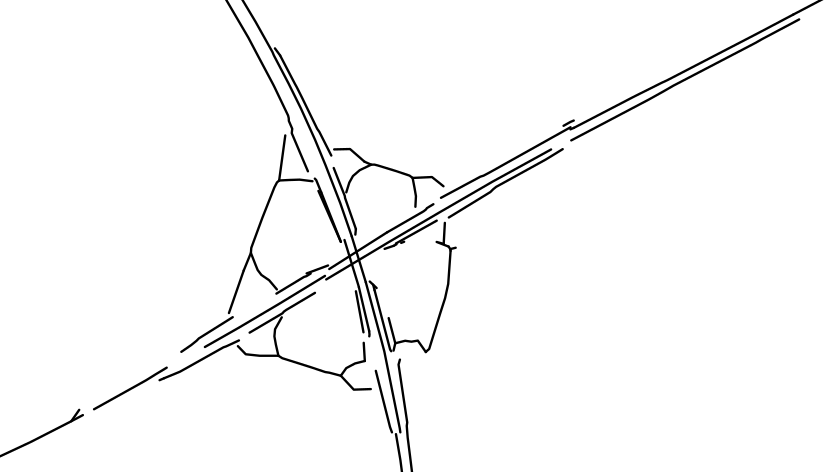
\includegraphics[width=\ScaleIfNeeded]{../chapter6/leverkusen-out}
	\caption{Überreste eines Kleeblatts nach zwei Generalisierungen (Autobahnkreuz Leverkusen)}
	\label{fig:iteration-gaps}
}

Die Anzahl der wiederholt durchzuführenden Generalisierungen kann im \term{Combiner} mit dem Schalter \texttt{--iterations} kontrolliert werden.

% evtl. beidseitig straßenbegleitende Fahrradwege zeigen (nur Erkennung)



\subsection{Eisenbahnstrecken}
\label{ch:result-railways}

Wie sich zeigt, ist die entwickelte Software grundsätzlich auch auf Eisenbahnstrecken anwendbar.
Beschränkt man sich auf Haupt- und Streckengleise (\osmtag{railway}[rail], \osmtag{usage}[main]) und berücksichtigt die Streckennummer als Attribut (\osmtag{ref}[*]), so werden viele doppelgleisige Streckenabschnitte erkannt und zusammengefasst.

Abbildung~\ref{fig:rail-kalk-out} zeigt das Ergebnis der Anwendung auf die südliche Einfahrt zum Güterbahnhof Köln-Kalk (\textfiguremark{1}).
Während die Reisezug-Gleise \textfiguremark{2}--\textfiguremark{3} und auch die drei Zulaufstrecken \textfiguremark{4}, \textfiguremark{5} und \textfiguremark{6} korrekt generalisiert wurden, funktioniert die Zuordnung im Weichenbereich bei \textfiguremark{7} nicht richtig, weil sich hier Gleise mit unterschiedlichen Streckennummern kreuzen.

Dem für ein Straßennetz entwickelten Verfahren zur Beseitigung von Topologielücken aus Abschnitt~\ref{ch:relocateGeneralisedNodes} gelingt es aufgrund der spitzen Winkel nicht, „geeignete“ Punkte zur Beseitigung der Lücken zu finden, wodurch ein gelungenes Ergebnis verhindert wird (Abbildung~\ref{fig:rail-kalk-detail}).

\twofigures{h}{
	\begin{overpic}[width=\ScaleIfNeeded]{../chapter6/rail-kalk-out}
%		\put(0,0){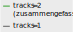
\includegraphics{../chapter6/legend-rail-out}}
	\end{overpic}
	% TODO: QGIS-export, ~10° rotiert
	\caption{Generalisierungsergebnis bei Anwendung des \term{Combiners} auf Bahnstrecken}
	\label{fig:rail-kalk-out}
}{
	\begin{overpic}[width=\ScaleIfNeeded]{../chapter6/rail-kalk-detail}
%		\put(0,0){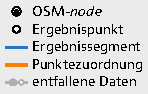
\includegraphics{../chapter6/legend-nodematch-gen}}
	\end{overpic}
	% TODO: QGIS-export, ~60° rotiert
	\caption{Detaildarstellung Generalisierung im Weichenbereich (\textfiguremark{7}~in Abbildung~\ref{fig:rail-kalk-out})}
	\label{fig:rail-kalk-detail}
}

Anders als im Straßennetz existieren derartige Probleme im Eisenbahnnetz nicht nur an Kreuzungen, sondern auch über längere Streckenabschnitte hinweg.
Betroffen sind insbesondere langgestreckte Überwerfungsbauwerke sowie Strecken mit Richtungsbetrieb.
Bei letzteren liegt zwischen den beiden zusammenzufassenden Gleisen mit derselben Streckennummer jeweils ein Gleis einer Strecke mit einer \emph{anderen} Nummer. \cf{wp:Richtungsbetrieb}

Auffallend ist ferner, dass der Zeitbedarf des \term{Combiners} für Bahnstrecken wesentlich höher ist als im Straßennetz.
Für Bahnstrecken in Köln werden mehr als 20~Segmente als „nah“ (im Sinne von \textproc{NaheSegmente} in Abschnitt~\ref{ch:split-algorithm}) beurteilt.
Dies liegt daran, dass Eisenbahngleise oft gebündelt verlegt werden, offenbar um angesichts der großen Kurvenradien den Platzbedarf zu minimieren.
Folglich sind auch entsprechend mehr Teilungen von Segmenten notwendig;
die Annahme $|S'| \approx 2 \cdot |S|$ aus Abschnitt~\ref{ch:algorithm-overview} ist selbst mit der Beschränkung auf Hauptgleise nicht mehr zutreffend.

Tabelle~\ref{tab:profiling-railways} zeigt, dass sich der Zeitbedarf durch bessere Anpassung der Definition von \textproc{Parallel} aus Abschnitt~\ref{ch:analyse-algorithm} auf die Bedingungen im Eisenbahnnetz zumindest geringfügig verbessern lässt.

\onetable{h}{
	\begin{tabular}{lrcrlcccrc}
& \multicolumn{2}{@{}c@{}}{\textproc{Parallel}} &&& \multicolumn{2}{@{}c@{}}{Wachstumsfaktor} &&& \\
Spezialfall & \multicolumn{1}{c}{$\alpha$} & $\eta$ & \multicolumn{1}{c}{$|S|$} & \multicolumn{1}{c}{$t$} & für $|S|$ & für $t$ & $\frac{|S'|}{|S|}$ & \multicolumn{1}{c}{$\nu$} & $\psi$ \\
\hline\rule{0mm}{0.8\normalbaselineskip}%
Straßen    & 15\degree & 40\,m &  8776 & 0,78\,s & --  & -- & 1,48 &  8 & 1,25 \\
Bahngleise & 15\degree & 40\,m & 11607 & 8,2\,s  & 1,3 & 11\hphantom{,2} & 2,81 & 22 & 1,77 \\
Bahngleise &  8\degree & 15\,m & 11607 & 2,5\,s  & 1,3 & \hphantom{1}3,2 & 2,14 & 11 & 1,66 \\
	\end{tabular}
	\caption{Zeitbedarf für unterschiedliche Spezialfälle und \textproc{Parallel}-Definitionen}
	\label{tab:profiling-railways}
}



% evtl. \subsection{Waldschneisen}



% single-chapter commands
\onlyinsubfile{\listoffigures}
\onlyinsubfile{\listoftables}
%\onlyinsubfile{% UTF-8

\documentclass[../main/thesis.tex]{subfiles}
\begin{document}

% include works in bibliography that aren't cited anywhere in the document (for debugging)
\onlyinsubfile{\nocite{*}}


\defbibnote{thesisBibIntro}{\justify%
Die Literaturangaben sind alphabetisch nach dem Kürzel sortiert.
Das Kürzel wird gebildet aus den ersten drei Buchstaben des Nachnamens des Autors, bei mehreren Autoren aus jeweils den Anfangsbuchstaben der Nachnamen, bei Körperschaften aus einer mnemonisch gewählten Folge von Kleinbuchstaben; jeweils ergänzt durch die letzten beiden Ziffern des Jahres der Veröffentlichung.
\par
Um ein eventuelles Nachschlagen zu erleichtern, sind die Referenzen wo immer möglich durch Angabe von Orten ergänzt, an denen eine Kopie des jeweiligen Werks am 1.~März 2018
% gegen 22~Uhr
aufzufinden war.
In der PDF-Ausgabe dieses Dokuments sind die URLs Hyperlinks.
Die Signaturen beziehen sich auf die Bibliothek des Karlsruher Instituts für Technologie und deren Standort „Fachbibliothek HsKA“.
\bigskip}


\RaggedRight
\addtocontents{toc}{\medskip}
\newpage\addcontentsline{toc}{chapter}{Literaturverzeichnis}
\printbibliography[title=Literaturverzeichnis,prenote=thesisBibIntro]

\end{document}
}
\end{document}


% TODO:
% fig:breitscheid-gen-styled - wie zentrieren und vernünftig umbrechen?
% fig:iteration-good - fehlende Punkte darstellen (als nodes, indem das Ergebnis der ersten Gen. als SHP importiert wird) und splitPts wegnehmen (bringen hier nicht mehr viel; evtl. auch Matches wegnehmen? eher ja.)
% fig:rail-kalk-out: neu
% fig:rail-kalk-detail: neu
% Legenden:
% - fig:result-trivial-detail-rolshover (rechts +splitPts, -nodes)
% - fig:koelnarena-gen-cleanup (+splitPts)
% - fig:kanal-gen-cleanup (+splitPts - oder splitPts hier schon wegnehmen? eher nicht.)
% - fig:iteration-good (unklar - erst Grafik neu)
% - fig:rail-kalk-out (fehlt)
% - fig:rail-kalk-detail (fehlt)
